\documentclass{article}
\usepackage[top=1in,left=1in, right = 1in, footskip=1in]{geometry}
\linespread{2}

\usepackage{amsthm}
\usepackage{amsmath}
\usepackage{amssymb}
\usepackage{amsfonts}

\usepackage{natbib}
\usepackage{hyperref}
\bibliographystyle{chicago}

\newcommand{\eref}[1]{(\ref{eq:#1})}
\newcommand{\fref}[1]{Fig.~\ref{fig:#1}}

\usepackage{color}
\newcommand{\comment}[3]{\textcolor{#1}{\textbf{[#2: }\textsl{#3}\textbf{]}}}
\newcommand{\swp}[1]{\comment{magenta}{SWP}{#1}}

\newcommand{\tsub}[2]{#1_{{\textrm{\tiny #2}}}}

\usepackage{graphicx}

\title{Practical guide to fitting SIR models}
\date{\today}
\author{Sang Woo Park}

\begin{document}
\maketitle

\pagebreak

\tableofcontents

\pagebreak


\section{Introduction}

Over the last few decades, a plethora of computational tools have been developed to study epidemic time series.
Central to these methods are mechanistic models.
These models allow us to study the qualitative dynamics of a system and infer underlying mechanisms that drove the observed patterns in the data.
For example, we now know that the complex dynamics of measles outbreaks were driven by seasonal transmission patterns \citep{earn2000simple}.

%% read https://www.ncbi.nlm.nih.gov/pmc/articles/PMC2607466/

The SIR model is one of the most basic mechanistic models. It describes how individuals move from susceptible ($S$) to infected ($I$) and to recovered ($R$) states in a homogeneously mixing population:
\begin{equation}\label{eq:sir}
\begin{aligned}
\frac{dS}{dt} &= b(t) - \left(\beta(t) \frac{I}{N} + \mu \right) S\\
\frac{dI}{dt} &= \beta(t) S \frac{I}{N} - (\gamma + \mu) I\\
\frac{dR}{dt} &= \gamma I - \mu R
\end{aligned}
\end{equation}
where $b(t)$ is the natural birth rate (or recruitment rate to susceptible population), $\beta(t)$ is the transmission rate, $\gamma$ is the recovery rate, and $\mu$ is the natural death rate.
Despite its simplicity, the SIR model is still widely used to study outbreaks, such as measles, plague, HIV, and influenza.
The main difficulty in analyzing these systems comes from estimating transmission rate, $\beta(t)$.

One way to estimate $\beta(t)$ is by matching the deterministic solution of the system \eref{sir} with the observed number of cases by minimizing sum of squares difference or negative log-likelihood.
This method is referred to as trajectory matching.
Similarly, it is possible to match gradients of the system \eref{sir} given if all state variables are observed.
Unlike trajectory matching, gradient matching does not require parametric forms of the rates to be specified beforehand and allows for flexible modeling of the system.
While these methods are computationally efficient and easy to implement, they do not allow us to take demographic stochasticity into account explicitly.

On the other hand, Monte Carlo methods allow us to model \emph{all} sources of variation (e.g., observation error and process error) explicitly.
Sequential Monte Carlo methods (e.g., particle filtering)


This is not at all an exhaustive list of all existing methods.
Generalized profiling balances bewteen trajectory matching and gradient matching by fitting a deterministic model  \citep{hooker2010parameterizing}.
Laplace approximation based methods are also available.

Of all these methods, the time series SIR (TSIR) method has been particularly successful in studying dynamics of ??? diseases, especially measles.




There are many ways to estimate underlying parameters of the SIR model \eref{sir};
yet their differences are unclear because they all rely on different set of assumptions.
Which one should one use?
Here, we compare TSIR each method against simulated data and study how differences in the assumptions affect our conclusions.
Then, we apply each method to measles time series from Boston and discuss implications.

\pagebreak

\section{Data}

Epidemic time series can be classified into three categories: incidence, mortality, and prevalence.
Incidence in defined as the number of newly infected individuals generated between two reporting periods.
Then, true incidence of the SIR model \eref{sir} between time $t$ and $t-\tsub{t}{rep}$, where $\tsub{t}{rep}$ is the length of reporting step, can be obtained by integrating total infection rate:
\begin{equation}
\int_{t-\tsub{t}{rep}}^{t} \beta(s) S \frac{I}{N} ds.
\end{equation}
Similarly, mortality case, which is defined as the number of individuals that died between two periods, can be obtained by integrating total death rate:
\begin{equation}
\int_{t-\tsub{t}{rep}}^{t} \gamma I ds.
\end{equation}
Finally, prevalence is defined as the number of infected individuals in the population and corresponds to the state variable $I$.
Number of reported incidence, mortality, and prevalence can be drawn from a binomial distribution with reporting rate $\rho$ and their corresponding true values given above.

When reporting period is equal to mean generation time, incidence and prevalence are often assumed to be equivalent (\fref{incidence}).
Indeed, for the simple SIR model \eref{sir}, it can be shown that incidence, prevalence, and mortality are similar to each other under Euler approximation when reporting period is equal to mean generation time (see Appendix).
However, this is not necessarily true for more complicated models. 
For a more realistic model with exposed period (SEIR model), incidence is similar to prevalence when reporting period is equal to mean \emph{generation time} whereas mortality is similar to prevalence when reporting period is equal to mean \emph{infectious period}. \swp{TODO: confirm}


\begin{figure}[t]
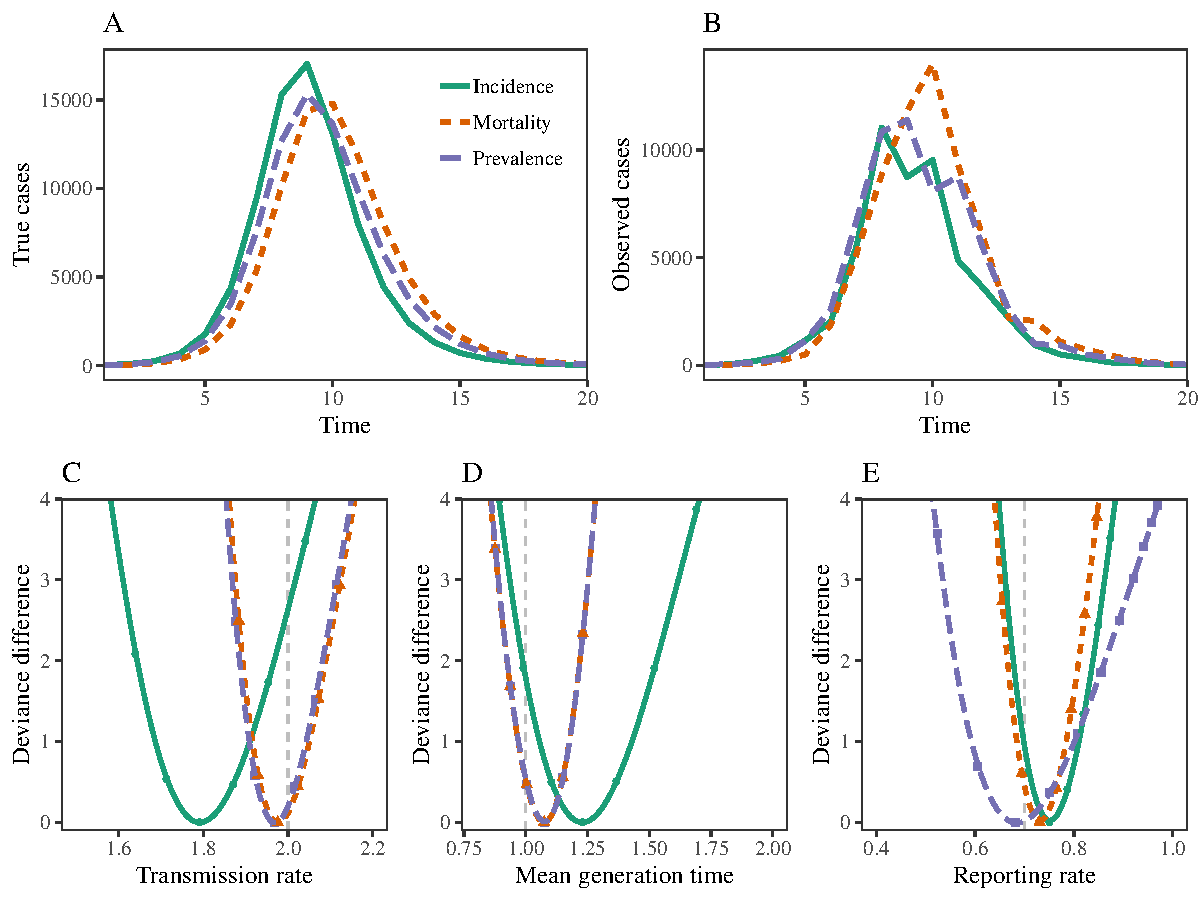
\includegraphics[width=\textwidth]{../figure/compare_profile_likelihood.pdf}
\caption{
\swp{TODO}
} 
\label{fig:incidence}
\end{figure}

Even if incidence, mortality, and prevalence \emph{data} are expected to be similar to each other when reporting period is equal to mean generation time, it is important to distinguish them when we are estimating underlying parameters of the SIR model, especially when mean generation time $1/\gamma$ is not exactly known.
To demonstrate this idea, we take a simulated epidemic time series and try to estimate transmission rate $\beta$, recovery rate $\gamma$, reporting rate $\rho$, and initial number of infected individuals $I(0)$ by sequentially treating the same time series as incidence, mortality, and prevalence report (\fref{incidence}).
We find that fitting prevalence and mortality yields almost identical estimates of the transmission rate $\beta$ and the recovery rate $\gamma$ whereas fitting incidence and mortality yields consistent estimates of the reporting rate $\rho$.

There is a simple explanation for these observations. 
As mortality is approximately a lagged reflection of prevalence regardless of reporting period (reported mortality case at time $t$ is approximately equal to $\rho \gamma I(t-\tsub{t}{rep}) \tsub{t}{rep}$), 
it is possible to generate a mortality curve that matches its corresponding prevalence curve by adjusting the reporting rate $\rho$.
Incidence report no longer  prevalence when reporting period is not equal to the mean generation time (i.e., when $\gamma$ is being estimated); therefore, fitting incidence curve yields a different estimate of the dynamical parameters, $\beta$ and $\gamma$, from fitting mortality or prevalence curves.
On the other hand, fitting incidence and mortality curve yields similar estimates of the reporting rate $\rho$ because they both contain equivalent information about the final size of an epidemic: total \emph{true} incidence and total \emph{true} mortality is equal to the final size of an epidemic.

\swp{Add transition...}

\pagebreak

\section{TSIR model}

\subsection{Model}

The time-series SIR (TSIR) method was developed by \cite{bjornstad2002dynamics} to estimate seasonally varying transmission rates of measles.
It relies on reconstructing the susceptible dynamics from birth and case reports and using linear regression, conditional on knowing ``true susceptible dynamics'', to estimate transmission rates.
Initial conditions are often estimated to improve goodness of fit.
%% something about initial step

The TSIR method begins by discretizing the infection process, assuming that disease generation-time is equal to reporting interval:
\begin{equation}
\begin{aligned}
S_{t+1} &= B_t + S_t - I_{t+1}
I_{t+1} &= \beta_t S_t \frac{I_t^\alpha}{N_t}
\end{aligned}
\end{equation}
where $\alpha$ is often referred to as a conversion factor from continuous-time model to discrete-time model or a heterogeneity parameter [CITE].
True incidence, $I_t$, is inferred from the observed incidence, $y_t$, and estimated reporting rate $\rho_t$: $I_t = y_t/\rho_t$.
Taking log on both sides, estimation of transmission rates $\beta_t$ becomes a regression problem:
\begin{equation}
\log I_{t + 1} = \log \beta_t + \log S_t + \alpha \log I_t - \log N_t + \epsilon_t.
\end{equation}

The estimation process is deterministic, but the TSIR method is analogous to fitting a stochastic model: 
equation ?? models step-ahead prediction as a function of previous state and process error, $\epsilon_t$. 
Coupled with a deterministic susceptible reconstruction and estimation of reporting rate, the TSIR method attributes all errors to one-step process noise and oversmooths the likelihood surface (figure ?).
Several studies have associated dynamics of the deterministic model (equation ??) with the inferred parameters from the regression but they are intrinsically different models.

\subsection{Probability of infection}

The TSIR model assumes that probability of infection is a nonlinear function of prevalence: $\beta I^\alpha/N$.
This contrasts with the linear assumption of the Euler approximation ($\beta I/N$) or the exponenital assumption of the hazard-based approximation ($1 - \exp(- \beta I/N)$).
Inclusion of the parameter $\alpha$ has been previously attributed to heterogeneity in the population or changes from continuous to discrete time model.
However, there is still a room for clearer understanding of the actual role of the parameter $\alpha$:
for example, a few studies recognize that the estimated $\alpha$ does not always correspond to the best predictive $\alpha$ and resorted to assuming $\alpha = 0.97$.

Glass et al derived an analytical expression for optimal values of $\alpha$ by comparing the changes in the infected population at equilibrium using a second order Taylor expansion. 
Based on their approximation, optimal value of $\alpha$ equals 1 when there is no birth term.
Instead, when we rewrite the TSIR model as 
\begin{equation}
\log \left(\frac{I_{t+1}}{S_t}\right) = \log\left(\frac{\beta I_t^\alpha}{N_t}\right) + \epsilon_t.
\end{equation}
it becomes much clearer that the TSIR model is trying to match the log probability of infection (when an epidemic is ongoing, changes in the susceptible population $S_t$ through natural birth or death is negeligible over a generation, and $I_{t+1}/S_t$ can be interpreted as the probability of infection over a generation). 
Then, we almost always expect $\alpha$ to be less than one because we expect the probability of infection (i.e., probability of finding a new host) to experience density dependence.

Though the difference in the interpretation of $\alpha$ is subtle, this perspective allows us to derive a useful connection between the discrete-time model and the continuous-time model.
A naive estimate of basic reproductive number from the TSIR model is $\beta$.
However, as discussed earlier, we often prefer to use hazard-based approach to approximate the continuous-time model. 
Then, we can find $\hat \beta$ such that $1 - \exp(-\hat\beta I/N)$ matches $\beta I^\alpha/N$ and use $\hat \beta$ as our estimate of the basic reproductive number instead.
A simple way to match two functions is to match their values at the mean observed incidence.
This corrections reduces bias in the estimate of the reproductive number by a large amount.

\subsection{Susceptible reconstruction}

One of the main assumptions behind the TSIR model is that the dynamics susceptible population $S_t$ must be known.
Assuming that all newborn infants become infected eventually, it is possible to recover the reporting rate, $\rho_t$, as well as the dynamics of the susceptible population as a deviation from its mean, $Z_t = S_t - \bar{S}$, by fitting a regression model to between cumulative births and cumulative cases: 
\begin{equation}
\sum_{t=1}^N B_t = \sum_{t=1}^N \frac{C_{t+1}}{\rho_{t+1}} + Z_{t+1} - Z_1,
\end{equation}
where $C_t$ is the number of observed cases. 
Then, the mean susceptible population $\bar S$ can be estimated using profile likelihood with the TSIR regression.

While this method of reconstructing the susceptible dynamics has been successfully used with the TSIR method, 
several questions remain to be answered.
First, how sensitive is our inference to regression methods?
Second, does $Z_t$ represent deviation from the overall population mean $\bar{S}$ or from some sort of moving average (assuming that population changes over time)?
Likewise, how does changes in population size or reporting rate over time affect our estimate of $\rho_{t+1}$ or $Z_t$?
Finally, how do assumptions about the population size affect estimate of the transmission rate?

\begin{figure}
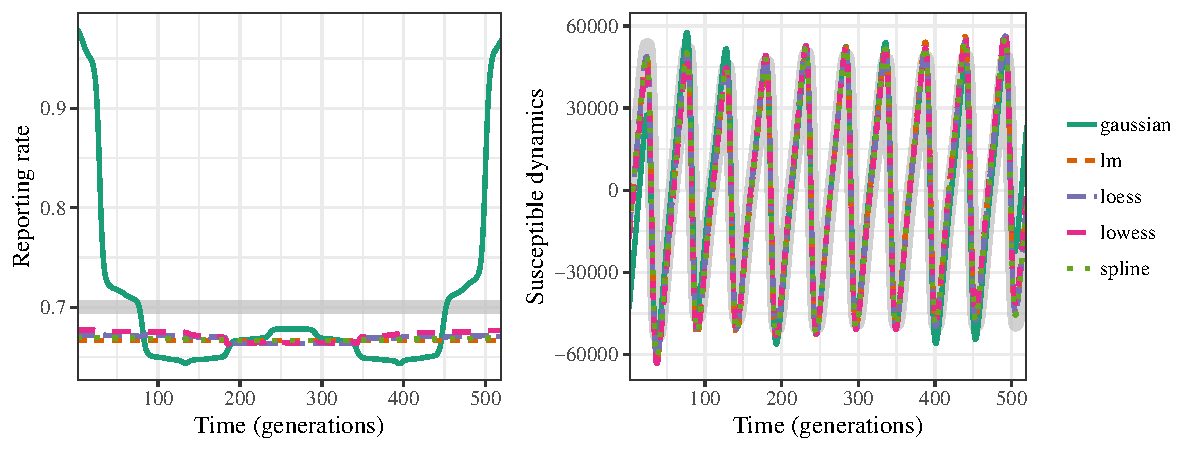
\includegraphics[width=\textwidth]{../figure/susceptible_reconstruction_tsir.pdf}
\caption{
\swp{TODO}
}
\label{fig:tsirrecon}
\end{figure}

First, we simulate an epidemic using the continuous deterministic SIR model for 10 years and introduce 70\% reporting rate.
Then, we use 5 different regression models available from the \texttt{tsiR} package and test their ability to infer reporting rate and susceptible dynamics (\fref{transmission}).
We find that estimates of transmission rates are highly sensitive to regression methods.
All nonlinear regression methods, especially guassian regression, yield inaccurate estimates near the beginning and the end of a time series.
Both linear and spline regressions provide reasonably accurate estimates.
In general, estimates of susceptible dynamics appear to be robust regardless of the regression method.



\subsection{Splines}



\pagebreak

\section{Other fitting methods}

\subsection{Trajectory matching}

\subsection{Gradient matching}

\subsection{Particle filtering}

\subsection{Renewal equation}

\pagebreak

\section{Numerical comparison of different methods}

\subsection{Single outbreak}

\subsection{Time-varying transmission rate}

\pagebreak

\section{Case study}

\section{Discussion}

\pagebreak

\section{Appendix}

\subsection{Equivalence of incidence, mortality, and prevalence}

First, recall that mortality case can be written as
\begin{equation}
\int_{t-\tsub{t}{rep}}^{t} \gamma I ds.
\end{equation}
When reporting period is equal to mean generation time, i.e., $\tsub{t}{rep} = 1/\gamma$, 
it follows that:
\begin{equation}
\int_{t-\tsub{t}{rep}}^{t} \gamma I ds \approx \gamma I(t-\tsub{t}{rep}) \tsub{t}{rep} = I(t-\tsub{t}{rep})
\end{equation}
Likewise, we can derive a similar relation for incidence:
\begin{equation}
\begin{aligned}
I(t+\tsub{t}{rep}) &= I(t) + \int_{t}^{t+\tsub{t}{rep}} \frac{dI(s)}{ds} ds\\
&= I(t) + \int_{t}^{t+\tsub{t}{rep}} \beta(s) S \frac{I}{N} ds - \int_{t}^{t+\tsub{t}{rep}}\\
&\approx \int_{t}^{t+\tsub{t}{rep}} \beta(s) S \frac{I}{N} ds
\end{aligned}
\end{equation}
Here, we assumed that individuals leaving infected class $I$ from natural mortality is negligible over the reporting period.

\swp{TODO}


\section{Fitting continuous models}

\subsection{Trajectory matching}

Trajectory matching is one of the simplest fitting methods.
As its name suggests, the goal is to find a set of parameters such that the deterministic trajectory of the ODE model best matches the observed data.
This method assumes that there is only measurement error and no process error.
The measurement model can be written as:
\begin{equation}
y_t \sim \mathrm{NegBinomial}\left(\mu_t= \int_{t-\Delta t}^{t} \beta(s) S \frac{\hat{I}}{N} ds, \phi \right),
\end{equation}
where $\rho$ is reporting rate and $\phi$ is dispersion parameter.
We prefer this model compared to the binomial or beta-binomial model because fitting binomial or beta-binomial models may not work if there are any irregular patterns in the data.

\subsection{Gradient matching}

\begin{figure}[t]
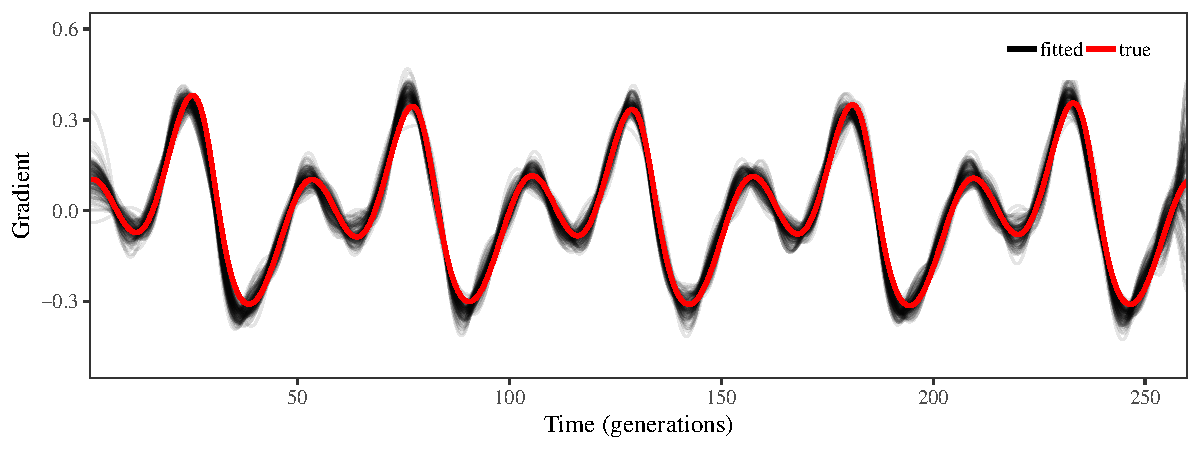
\includegraphics[width=\textwidth]{../figure/gradient_matching_sinusoidal.pdf}
\caption{This is not a caption.}
\end{figure}

When \emph{all} state variables are observed, we can fit smooth curves to the data and obtain an estimate of the gradients of the ODE by taking the derivatives of the estimated smooth functions.
Gradient matching methods seek to estimate the rate equation using nonparametric regression.
However, for most epidemics, it is impossible to have data of all state variables.
When only incidence is provided, we have no direct observations of any state variables. 
If we can reconstruct the dynamics of the susceptible population and assume that incidence is sufficiently similar to prevalence, we can still be able to apply gradient mathing methods.

Observe that
\begin{equation}
\frac{d \log\hat{I}}{dt} = \beta(t) \frac{S}{N} - (\gamma + \mu),
\end{equation}
If we can obtain a reasonable estimate of the gradient $Z_i = d \log \hat{I}/dt (t_i)$, we can write
\begin{equation}
Z_i + (\gamma + \mu) = \exp \left(\log \beta (t_i) + \log S_i - \log N \right)  + \epsilon_i
\end{equation}
and estimate $\beta$, given that we can reconstruct the susceptible dynamics $S_i$.
Estimate of $\beta$ can be done using nonparametric regression by treating $\log S_i$ and $\log N$ as offset terms.

First, we want to test whether gradients can be reliably estimated from incidence data alone by simulating a deterministic SIR model with measurement error.
We use natural cubic spline with knots placed every 6 biweeks.
It works generally well but there is systematic bias.
When gradients are at their local maxima (and minima), we tend to overestimate (and underestimate) the gradients.
This is because incidence precedes prevalence???

If we simply construct confidence intervals based on equation ?? we underestimate uncertainty significantly by ignoring the uncertainty in the estimated gradients $Z_i$.

Conditions:
\begin{itemize}
	\item See Jost and Ellner (???)
	\item sampled sufficiently
	\item not too much error
	\item Brunel Parameter estimation of ODE’s via nonparametric estimators
\end{itemize}


%% read pomp-Astic somewhere

\subsection{Generalized profiling}

Generalized profiling combines trajectory matching with gradient matching.

\subsection{Spectral matching}

What is this? Read Reuman et al. 2006
%% https://www.pnas.org/content/pnas/103/49/18860.full.pdf

\section{Fitting discrete time models}

\subsection{Particle filtering}

Particle filtering provides a way of approximating the likelihood for stochastic models.
In this paper, we focus on mif2 method.

\begin{equation}
\begin{aligned}
S_{t + \Delta t} &= B_t + S_t - S_t \left(1- \exp\left(-\beta_t \frac{I_t}{N_t} \Delta t\right)\right)\\
I_{t + \Delta t} &= S_t \left( 1- \exp\left(-\beta_t \frac{I_t}{N_t} \Delta t\right)\right) + I_t - I_t (1 - \exp(-(\gamma + \mu) \Delta t))
\end{aligned}
\end{equation}
Tries to account for variation in ... but still ... When are these assumptions appropriate?

\subsection{Incidence-based models}

\cite{li2018fitting} compared incidence-based models across several Bayesian platforms.
In our case, we can write a similar model as:
\begin{equation}
\begin{aligned}
S_{t + \Delta t} &= B_t + S_t - I_{t+\Delta t}\\
\phi_t &= \sum_{i=1}^\ell k(i) I_{t - \ell +i}\\
I_{t + \Delta t} &\sim \mathrm{BetaBin}(1- e^{-\phi_t}, S_t,\delta_P)\\
\mathrm{Obs}_t &\sim \mathrm{NegBin}(P_{rep}, \sum I_t, \delta_{obs})
\end{aligned}
\end{equation}
When reporting period is same as the mean generation time, we want to simulate the model on a finer scale.

Disadvantage: unable to model mechanisms; difficult to deal with prevalence or mortality data.
Advantage: flexible generation time distribution.



\section{Results}

\subsection{Statistical inference}

\begin{figure}[t]
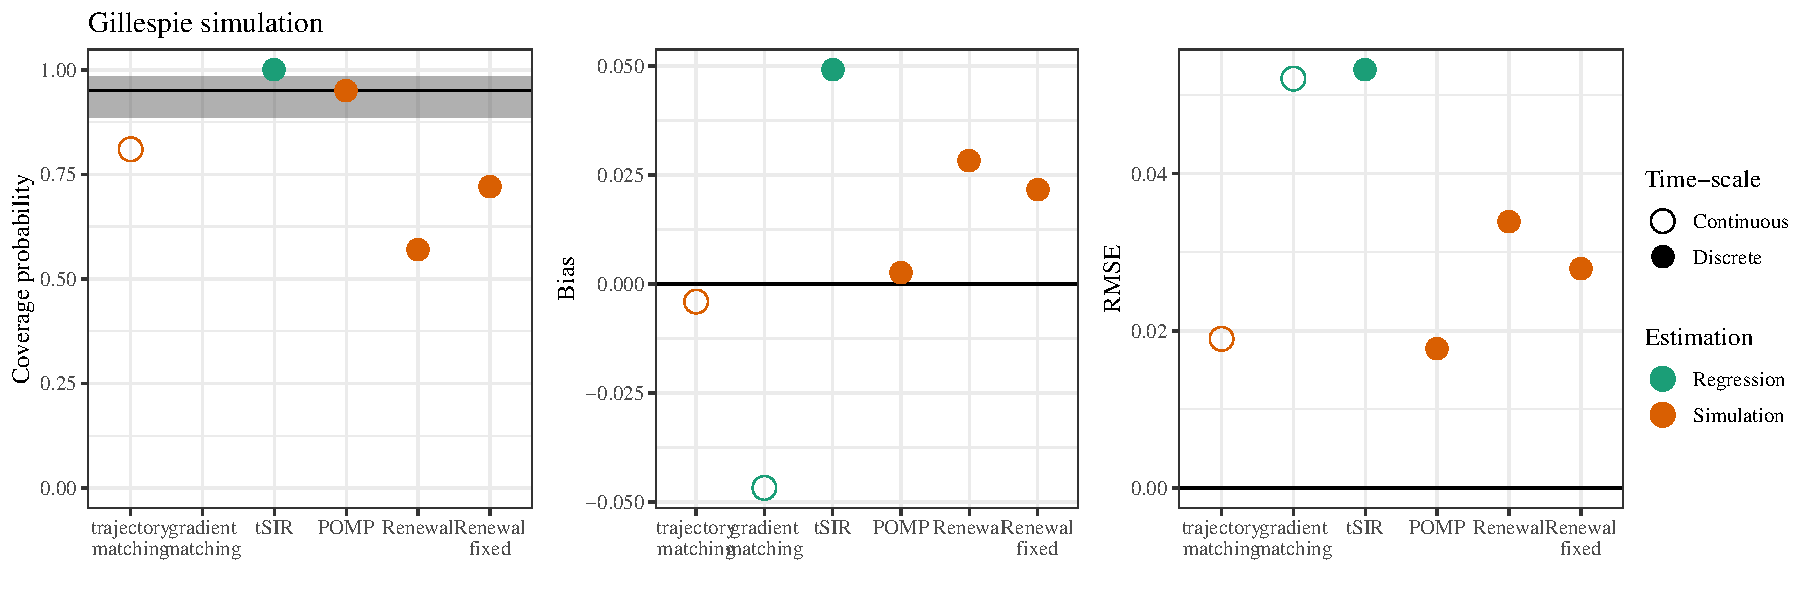
\includegraphics[width=\textwidth]{../figure/compare_estimate_sir.pdf}
\end{figure}



\bibliography{thesis}

\pagebreak

\section{Appendix}

\subsection{Derivation of growth rate in discrete-time SIR model}


Derivation:
\begin{equation}
\begin{aligned}
S_{t+\Delta t} &= S_t - S_t (1- \exp(-\beta I_t \Delta t/N))\\
I_{t+\Delta t} &= S_t (1- \exp(-\beta I_t \Delta t/N)) + I_t - I_t (1- \exp(-\gamma \Delta t))
\end{aligned}
\end{equation}
Assuming tat $S_t$ is approximately equal to $N$, we get
\begin{equation}
I_{t+\Delta t} = N_t (1- \exp(-\beta I_t \Delta t/N)) + I_t \exp(-\gamma \Delta t)
\end{equation}
When $I_t \approx 0$, $\exp(-\beta I_t \Delta t/N) \approx 1 - \beta I_t \Delta t/N$ and so
\begin{equation}
\begin{aligned}
I_{t+\Delta t} &\approx  I_t \beta \Delta t + I_t \exp(-\gamma \Delta t)\\
&= I_t (\beta \Delta t + \exp(-\gamma \Delta t))
\end{aligned}
\end{equation}
Substituting $\hat{\gamma}$, we get
\begin{equation}
I_{t+\Delta t} = I_t \left(1 + \beta \Delta t - \frac{\Delta t}{\mu}\right),
\end{equation}
Therefore,
\begin{equation}
I_{t} = I_0 \left(1 + \beta\Delta t - \frac{\Delta t}{\mu}\right)^{t/\Delta t}
\end{equation}
and the initial growth rate is given by
\begin{equation}
r = \frac{1}{\Delta t} \log \left(1 + \beta \Delta t - \frac{\Delta t}{\mu}\right).
\end{equation}




\subsection{Probability of infection}

In both the TSIR model and the hazard-based model, transition from the susceptible comparment, $S$, to the infected compartment, $I$, is represented as a product of number of susceptible individuals and probability of infection between two time steps $t$ and $t + \Delta t$.
The TSIR model assumes that the probability of infection is a linear function of prevalence $I_t$.
This formulation is based on the Euler approximation to the solution of the ordinary differential equation.
On the other hand, the hazard-based model assumes that the probability of infection is an inverse exponential function of prevalence $I_t$.
Besides their differences in the relationship between prevalence and probability of infection, there are two more assumptions that we need to consider: (1) force of infection remains constant over two time steps and (2) new susceptible individuals have zero probability of infection between the two time steps.



\subsection{Infectious period}

Geometric distribution with probability of $1-\exp(-\gamma \Delta t)$ and unit of $\Delta t$.
Then, mean infectious period and generation interval is given by 
\begin{equation}
\frac{\Delta t}{1-\exp(-\gamma \Delta t)}.
\end{equation}
An important but often overlooked component is the variance of the distribution.
Squared coefficient of variation for this distribution is equal to $\exp(-\gamma \Delta t)$, which necessarily depends on pre-specified time-step $\Delta t$.
If we want to match the mean of the distribution to a fixed value $\mu$ regardless of our choices of $\Delta t$, we obtain 
\begin{equation}
\hat \gamma = - \frac{1}{\Delta t} \log\left(1 - \frac{\Delta t}{\mu}\right)
\end{equation}
Then,
\begin{equation}
\mathrm{CV}_{\tiny\textrm{Infectious period}}(\Delta t)^2 = 1 - \frac{\Delta t}{\mu}.
\end{equation}

We expect changes in variation in infectious period to affect variation in stochstic realizations.

This means that the relationship between $r$ and $\mathcal R$ changes.
For this generation-interval distribution, we have
\begin{equation}
\mathcal R = 1 + \frac{\exp(r) -1}{(1-\exp(-\gamma \Delta t)) }
\end{equation}
Substituting 
\begin{equation}
r = \frac{1}{\Delta t} \log \left(1 + \beta \Delta t - \frac{\Delta t}{\mu}\right),
\end{equation}
as well as $\hat \gamma$, we get
\begin{equation}
\mathcal R = 1 + \frac{\mu}{\Delta t} \left(1 + \beta \Delta t - \frac{\Delta t}{\mu}\right)^{1/\Delta t}
\end{equation}
Then, we can obtain a relationship between $\mathcal R$ of a discrete-time system and that of a corresponding continuous time system, assuming that contact rate $\beta$ and mean generation-time $\mu$ are the same:
\begin{equation}
\mathcal R_{\tiny \textrm{discrete}} = 1 + \frac{\mu}{\Delta t} \left(1 + \frac{(\mathcal R_{\tiny \textrm{continuous}}  - 1) \Delta t }{\mu}\right)^{1/\Delta t}
\end{equation}

On the other hand, we may want to match choose $\beta$ and $\mu$ to match true $r$ and $\mathcal R$.



\end{document}
